\documentclass[11pt,a4paper]{report}

% ------------------------------------------------------------------ packages
\usepackage[margin=2.5cm]{geometry}
\usepackage{graphicx}
\usepackage{booktabs}
\usepackage{amsmath,amssymb}
\usepackage{float}
\usepackage{caption}
\usepackage{subcaption}
\usepackage{array}
\usepackage{tabularx}
\usepackage{multirow}
\usepackage{xcolor}
\usepackage{enumitem}
\usepackage{listings}
\usepackage{fancyhdr}
\usepackage[hidelinks]{hyperref}

\graphicspath{{figures/}}
\setlist{itemsep=2pt,topsep=4pt}
\definecolor{codebg}{RGB}{245,245,245}
\lstset{basicstyle=\ttfamily\small,backgroundcolor=\color{codebg},frame=single,
        breaklines=true,columns=fullflexible,keepspaces=true,showstringspaces=false}
\newcommand{\best}[1]{\textbf{#1}}

\pagestyle{fancy}
\fancyhf{}
\lhead{CT-317 Machine Learning -- Complex Engineering Problem}
\rhead{\thepage}
\renewcommand{\headrulewidth}{0.4pt}

% =================================================================== title
\begin{document}
\begin{titlepage}
\centering
{\Large\bfseries DEPARTMENT OF SOFTWARE ENGINEERING\par}
\vspace{2pt}
{\large BACHELORS IN SOFTWARE ENGINEERING\par}
\vspace{1.2cm}
{\large Course Code: CT-317 \quad|\quad Course Title: Machine Learning\par}
\vspace{4pt}
{\large SE Batch 2023, Fall Semester 2026\par}
\vspace{2cm}
{\Huge\bfseries Complex Engineering Problem\par}
\vspace{0.4cm}
{\LARGE Term Project Report\par}
\vspace{1cm}
{\large
Q1. Fake-News Headline Classification with $k$-Nearest Neighbours\\[3pt]
Q2. Sentiment (Emotion) Analysis from Noisy Audio Recordings\\[3pt]
Q3. Surface Defect Detection, Classification and Localisation\par}
\vspace{2cm}
{\large\bfseries Group Members\par}
\vspace{6pt}
\renewcommand{\arraystretch}{1.6}
\begin{tabular}{|c|p{7.5cm}|p{3.5cm}|}
\hline
\textbf{Student No.} & \textbf{Name} & \textbf{Roll No.}\\ \hline
S1 & Sumayyah Mohammedy & SE-23013\\ \hline
S2 & Amna Khan & SE-23039\\ \hline
S3 & Mariha Mahmood & SE-23047\\ \hline
S4 & Haris Bin Nasir & SE-23084\\ \hline
\end{tabular}
\vspace{1cm}

{\large Source code: \url{https://github.com/hbnasir23/ml-cep-ct317}\par}
\vfill
{\large Submitted to: \rule{6cm}{0.4pt}\par}
\vspace{8pt}
{\large Date of submission: \rule{4cm}{0.4pt}\par}
\end{titlepage}
\pagenumbering{roman}

% ================================================================ abstract
\begin{abstract}
\noindent
This report covers the three machine-learning problems in the CT-317 Complex Engineering Problem.
\textbf{Q1} classifies 3,266 news headlines as real or fake with scikit-learn's
$k$-nearest-neighbour classifier on bag-of-words features. With the default Euclidean
distance the selected model ($k=12$) reaches 63.9\% test accuracy. Switching to cosine
distance raises this to \textbf{75.7\%}, because cosine distance ignores headline length and
compares only which words are used.
\textbf{Q2} recognises six emotions in 7,442 noisy speech clips (CREMA-D). Clips are
low-pass filtered at 4\,kHz, and 242 hand-crafted features are extracted (FFT bands, MFCCs,
mel-spectrogram, chromagram, spectral shape, prosody and bicoherence). Five classifiers are
evaluated on a \emph{speaker-independent} split. The best, an RBF-SVM, reaches
\textbf{52.4\%} accuracy on unseen speakers (chance is 16.7\%). Per-speaker feature
normalisation raises this to \textbf{61.3\%}.
\textbf{Q3} detects holes and pen marks in 1,500 high-resolution images of a paper reel.
The pipeline flattens uneven illumination, proposes dark candidate regions and describes
them with colour histograms, spatial binning, HOG, LBP, GLCM and shape descriptors.
Four classifiers reach \textbf{97--99\%} test accuracy. A region classifier trained with
hard negatives scores every proposal to localise the defect, and the chosen box lies on the
true defect in all inspected test images.
All code is modular and reproducible (fixed seeds, cached features). Each question can be
run with a single command. As an innovation, an \emph{explainable} web application lets
users test all three models with their own input (typed headlines, live microphone
recordings, uploaded images) and shows \emph{why} each model decided as it did.
The code is public at \url{https://github.com/hbnasir23/ml-cep-ct317}.
\end{abstract}

\tableofcontents
\listoffigures
\listoftables

% ============================================================ introduction
\cleardoublepage\pagenumbering{arabic}
\chapter{Introduction}

\section{Objectives}
The Complex Engineering Problem (CEP) asks for three complete machine-learning pipelines,
one in each of three application areas:
\begin{enumerate}
  \item \textbf{Classification (text).} Learn to use an existing library implementation
        (scikit-learn's \texttt{KNeighborsClassifier}), handle train/validation/test splits,
        and study the effect of the distance metric.
  \item \textbf{Natural-language and audio processing.} Select data, design suitable splits,
        remove noise with low-pass filtering, extract audio features identified in the
        literature, and compare KNN, Logistic Regression, Naive Bayes, SVM and a Neural
        Network.
  \item \textbf{Computer vision.} Design a classical feature pipeline (colour histogram,
        spatial binning, HOG and further features from the literature), compare SVM, Naive
        Bayes, Logistic Regression and a Neural Network for three-class defect
        classification, and localise defects with bounding boxes.
\end{enumerate}

\section{Tools and environment}
All work was done in Python~3.13 on Windows~11 (12 CPU cores) with
scikit-learn~1.8 \cite{sklearn}, NumPy, SciPy, pandas and matplotlib.
\texttt{librosa}~1.0 \cite{librosa} was used for audio analysis, and OpenCV~5.0 and
scikit-image~0.26 \cite{skimage} for image processing. The interactive demo uses
Streamlit. Exact package requirements are listed in \texttt{requirements.txt}.

\section{General methodology}
Three principles were applied to every question so that the reported numbers are trustworthy:
\begin{itemize}
  \item \textbf{Three-way split.} Hyper-parameters are chosen \emph{only} on a validation
        set. The test set is used exactly once, to report the final result.
  \item \textbf{No information leakage.} All pre-processing that learns from data
        (vocabulary, feature scaling) is fitted on the training data only. Splits are
        designed so that near-duplicate information (for example, the same speaker) cannot
        appear in both training and test data.
  \item \textbf{Reproducibility.} All random operations use seed 42, and expensive feature
        extraction is cached on disk so that every table and figure can be regenerated.
\end{itemize}

\section{Repository structure}
\begin{lstlisting}
ml_cep/
  README.md, requirements.txt, app.py   (Streamlit demo for all questions)
  q1/  q1_knn.py                         data/, results/, models/
  q2/  audio_features.py  q2_audio_sentiment.py  q2_extras.py  predict.py
       dataset_repo/ (CREMA-D clone), results/, models/, cache/
  q3/  defect_features.py  q3_defect_detection.py  predict.py  error_analysis.py
       data/out/{paper,hole,penMark}/, results/, models/, cache/
  report/  report.tex, figures/
\end{lstlisting}

% ===================================================================== Q1
\chapter{Q1: Classification with Nearest Neighbours}

\section{Problem statement}
The task is to classify news headlines as \emph{real} or \emph{fake} with scikit-learn's
\texttt{KNeighborsClassifier}. We must (a) load and vectorise the data and split it
70/15/15, (b) select $k\in\{1,\dots,20\}$ by validation accuracy with the default metric,
and (c) repeat the selection with \texttt{metric='cosine'} and explain the difference.

\section{Dataset}
The cleaned dataset in \texttt{hw1\_data.zip} contains 1,968 real headlines
(\texttt{clean\_real.txt}, from the ``million headlines'' corpus, restricted to headlines
containing ``trump'' after October 2016) and 1,298 fake headlines
(\texttt{clean\_fake.txt}, from the Kaggle fake-news dataset), 3,266 in total. The CSV
files in the same archive contain an unrelated regression dataset and are not used.

\section{Methodology}
\subsection{\texttt{load\_data}: pre-processing and splitting}\label{sec:q1load}
\begin{enumerate}
  \item Read both files and label them \texttt{real}=1 and \texttt{fake}=0.
  \item Make a \emph{stratified} random split into 70\% training, 15\% validation and
        15\% test data (2,286 / 490 / 490 headlines). Stratification keeps the real/fake
        ratio (60/40) the same in every subset.
  \item Fit a \texttt{CountVectorizer} on the \emph{training headlines only}, giving a
        vocabulary of 4,804 words, and transform all three subsets. Each headline becomes a
        sparse vector of word counts. Words that appear only in validation or test headlines
        are ignored, exactly as they would be for genuinely new data.
\end{enumerate}

\subsection{\texttt{select\_knn\_model}: model selection}
For every $k=1,\dots,20$, a \texttt{KNeighborsClassifier(n\_neighbors=k)} is trained with
all other arguments at their defaults (Minkowski distance with $p=2$, i.e.\ Euclidean;
uniform weights). Training and validation accuracy are recorded. The $k$ with the highest
validation accuracy is selected, with ties broken towards the larger (smoother) $k$. The
selected model's accuracy on the test set is then reported. Part~(c) repeats the procedure
with \texttt{metric='cosine'}.

\section{Results}\label{sec:q1res}
\begin{figure}[H]
  \centering
  \begin{subfigure}{0.49\textwidth}
    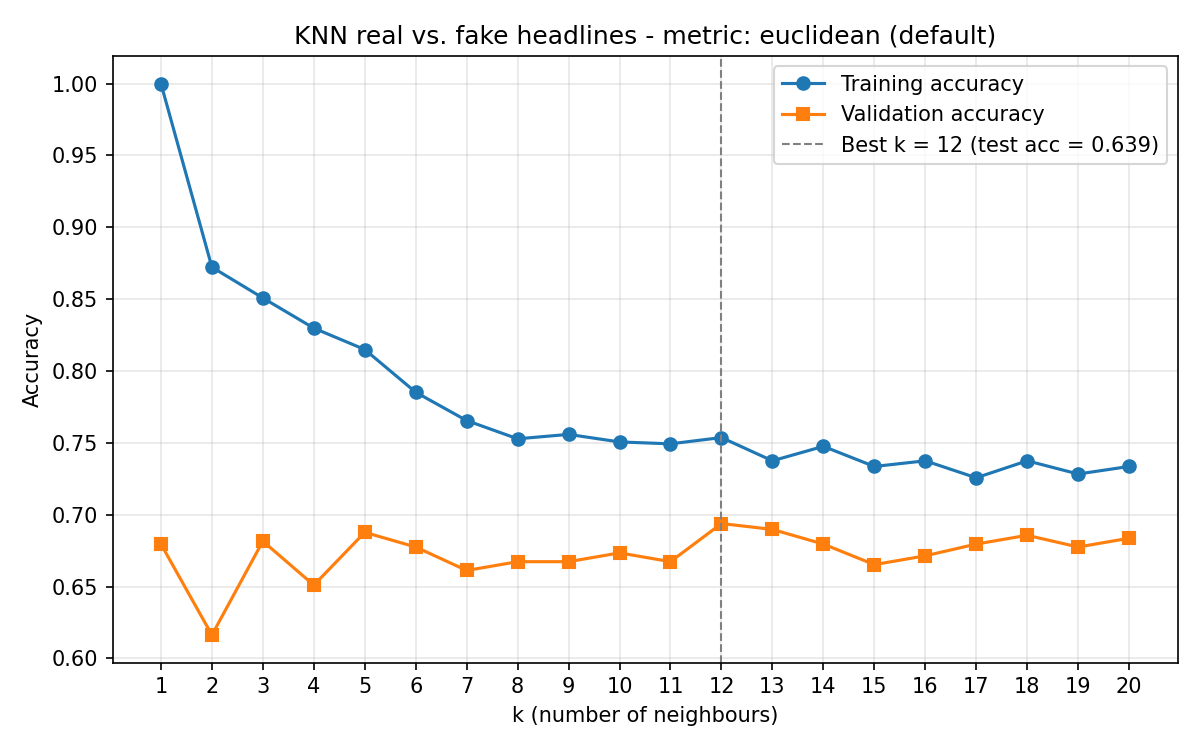
\includegraphics[width=\linewidth]{q1_euclidean.png}
    \caption{Euclidean (default) metric}
  \end{subfigure}
  \hfill
  \begin{subfigure}{0.49\textwidth}
    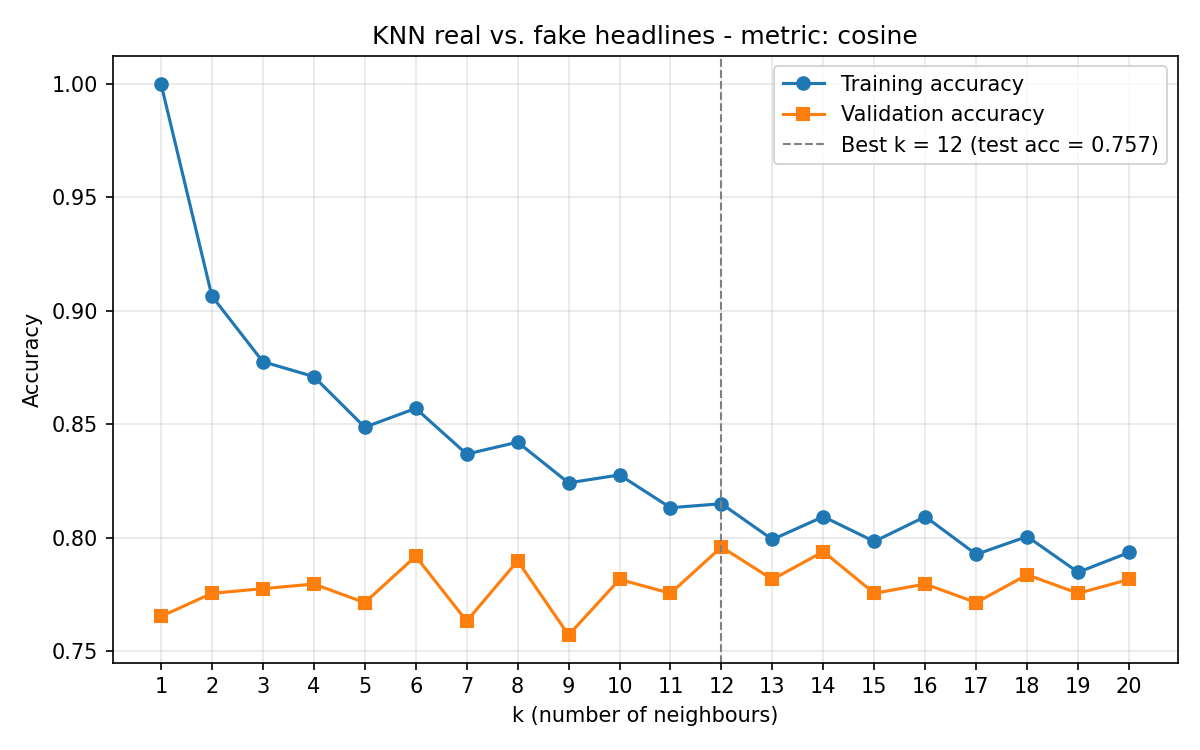
\includegraphics[width=\linewidth]{q1_cosine.png}
    \caption{Cosine metric}
  \end{subfigure}
  \caption{Training and validation accuracy of KNN as a function of $k$.}
  \label{fig:q1}
\end{figure}

\begin{table}[H]
  \centering
  \caption{Q1 model selection results.}
  \label{tab:q1}
  \begin{tabular}{lcccc}
    \toprule
    Metric & Best $k$ & Train acc. & Validation acc. & \textbf{Test acc.}\\
    \midrule
    Euclidean (default) & 12 & 0.754 & 0.694 & 0.639\\
    Cosine              & 12 & 0.815 & 0.796 & \best{0.757}\\
    \bottomrule
  \end{tabular}
\end{table}

\paragraph{Observations.}
With $k=1$ the training accuracy is 100\%: every training headline is its own nearest
neighbour, so the model memorises the data and over-fits (validation accuracy is only
0.680 for Euclidean and 0.765 for cosine). As $k$ grows, training accuracy falls and the
gap to validation accuracy narrows, which is the expected bias--variance trade-off. Cosine
distance is better than Euclidean for \emph{every} $k$ (Figure~\ref{fig:q1}), by about
10 percentage points on validation data and 11.8 points on the test set.

\section{Why does the cosine metric perform better?}\label{sec:q1cos}
\subsection{How \texttt{metric='cosine'} computes distance}
For two count vectors $\mathbf{u},\mathbf{v}$,
\begin{equation}
  d_{\cos}(\mathbf{u},\mathbf{v}) = 1-\frac{\mathbf{u}\cdot\mathbf{v}}{\lVert\mathbf{u}\rVert\,\lVert\mathbf{v}\rVert}
  = 1-\cos\theta,
\end{equation}
where $\theta$ is the angle between the vectors. The distance depends only on the
\emph{direction} of the vectors, i.e.\ on the relative proportions of the words, not on
their length. It is 0 for headlines with identical word proportions and 1 for headlines
with no word in common. The Euclidean distance
$d_E=\lVert\mathbf{u}-\mathbf{v}\rVert_2$ depends on both direction and magnitude.

\subsection{The hint dataset}
For \texttt{['cat', 'bulldozer', 'cat cat cat']} the count vectors over the vocabulary
(\textit{bulldozer}, \textit{cat}) are $(0,1)$, $(1,0)$ and $(0,3)$.
\begin{table}[H]
\centering
\caption{Distances for the hint dataset.}
\begin{tabular}{lcc}
\toprule
Pair & Euclidean & Cosine\\
\midrule
cat -- bulldozer & $\sqrt2 = 1.414$ & 1\\
cat -- cat cat cat & 2.000 & \best{0}\\
bulldozer -- cat cat cat & 3.162 & 1\\
\bottomrule
\end{tabular}
\end{table}
\noindent Under Euclidean distance, \emph{cat} is closer to \emph{bulldozer} than to
\emph{cat cat cat}, even though the latter is about the same thing. Cosine distance gives
the intuitive answer.

\subsection{Consequences for headlines}
\begin{itemize}
  \item Headlines have different lengths and some repeat words. Under Euclidean distance,
        short headlines are close to \emph{all} other short headlines regardless of topic
        (their vectors are all near the origin), and long headlines are far from everything.
        The neighbours are therefore chosen largely by length, which carries little
        information about real versus fake.
  \item Cosine distance normalises away the length and measures word \emph{overlap}. The
        nearest neighbours then share vocabulary (topic, named entities, sensational words
        typical of fake headlines), which is what separates the two classes.
  \item Bag-of-words vectors are very sparse and high-dimensional (4,804 dimensions,
        roughly 8 non-zeros each). In such spaces Euclidean distances concentrate and
        become less discriminative, whereas cosine similarity remains a meaningful
        measure of shared content. This is why it is the standard choice in information
        retrieval \cite{manning}.
\end{itemize}

% ===================================================================== Q2
\chapter{Q2: Sentiment Analysis from Audio Recordings}

\section{Problem statement}
The goal is to build a classifier that identifies the emotion expressed in a recorded
speech clip. The audio must first be de-noised with low-pass filtering. Features identified
in the literature are then extracted, and five classifiers are compared: KNN, Logistic
Regression, Naive Bayes, SVM and a Neural Network.

\section{Dataset}
The provided repository (a noisy version of CREMA-D \cite{cremad}) contains
\textbf{7,442} WAV clips (16\,kHz, mono, 16-bit, about 2--3\,s each) recorded by
\textbf{91 actors} (48 male, 43 female, aged 20--74, of diverse ethnicities). Each actor
reads 12 sentences with one of six emotions. Three of the four emotion-intensity levels
(low, medium, high) are used only for one sentence; the rest are ``unspecified''. File
names encode the metadata, e.g.\ \texttt{1001\_DFA\_ANG\_XX.wav} =
actor~1001, sentence DFA, \emph{Anger}, unspecified intensity. The classes are almost
balanced: 1,271 clips each for Anger, Disgust, Fear, Happy and Sad, and 1,087 for Neutral.

\section{Data selection and splitting}\label{sec:q2split}
The emotion classifier must work on speakers it has never heard. If clips were split at
random, every actor would appear in both training and test data, and the classifier could
partly recognise the \emph{voice} instead of the \emph{emotion}, giving over-optimistic
results. We therefore use a \textbf{speaker-independent} split: the 91 actors (not the
clips) are divided randomly 70/15/15 with \texttt{GroupShuffleSplit}. The code asserts
that the three actor sets are disjoint. All clips are used, all six emotions are present in
every split in the original proportions, and all 12 sentences appear in every split
(Table~\ref{tab:q2split}).

\begin{table}[H]
\centering
\caption{Speaker-independent split of CREMA-D.}
\label{tab:q2split}
\begin{tabular}{lcccccccc}
\toprule
Split & Actors & ANG & DIS & FEA & HAP & NEU & SAD & Total\\
\midrule
Train & 63 & 880 & 880 & 880 & 880 & 752 & 880 & 5,152\\
Validation & 14 & 195 & 195 & 195 & 195 & 167 & 195 & 1,142\\
Test & 14 & 196 & 196 & 196 & 196 & 168 & 196 & 1,148\\
\bottomrule
\end{tabular}
\end{table}

\section{Pre-processing: noise removal}\label{sec:q2pre}
\begin{enumerate}
  \item \textbf{Low-pass filtering.} A 6th-order Butterworth low-pass filter with a cut-off
        of \textbf{4\,kHz} is applied in second-order sections with \texttt{sosfiltfilt}
        (forward--backward). The result therefore has zero phase distortion, so the timing
        of pitch and energy contours is preserved. Speech intelligibility and most
        prosodic and emotional cues lie below 4\,kHz \cite{rabiner}, while the added
        broadband noise extends up to the 8\,kHz Nyquist frequency, so the filter removes
        about half of the noise band while keeping the speech.
  \item \textbf{Silence trimming} of leading and trailing segments more than 30\,dB below
        the peak, so that statistics are computed over speech only.
  \item \textbf{Peak normalisation}, so that loudness differences caused by recording gain
        do not dominate.
\end{enumerate}

\begin{figure}[H]
  \centering
  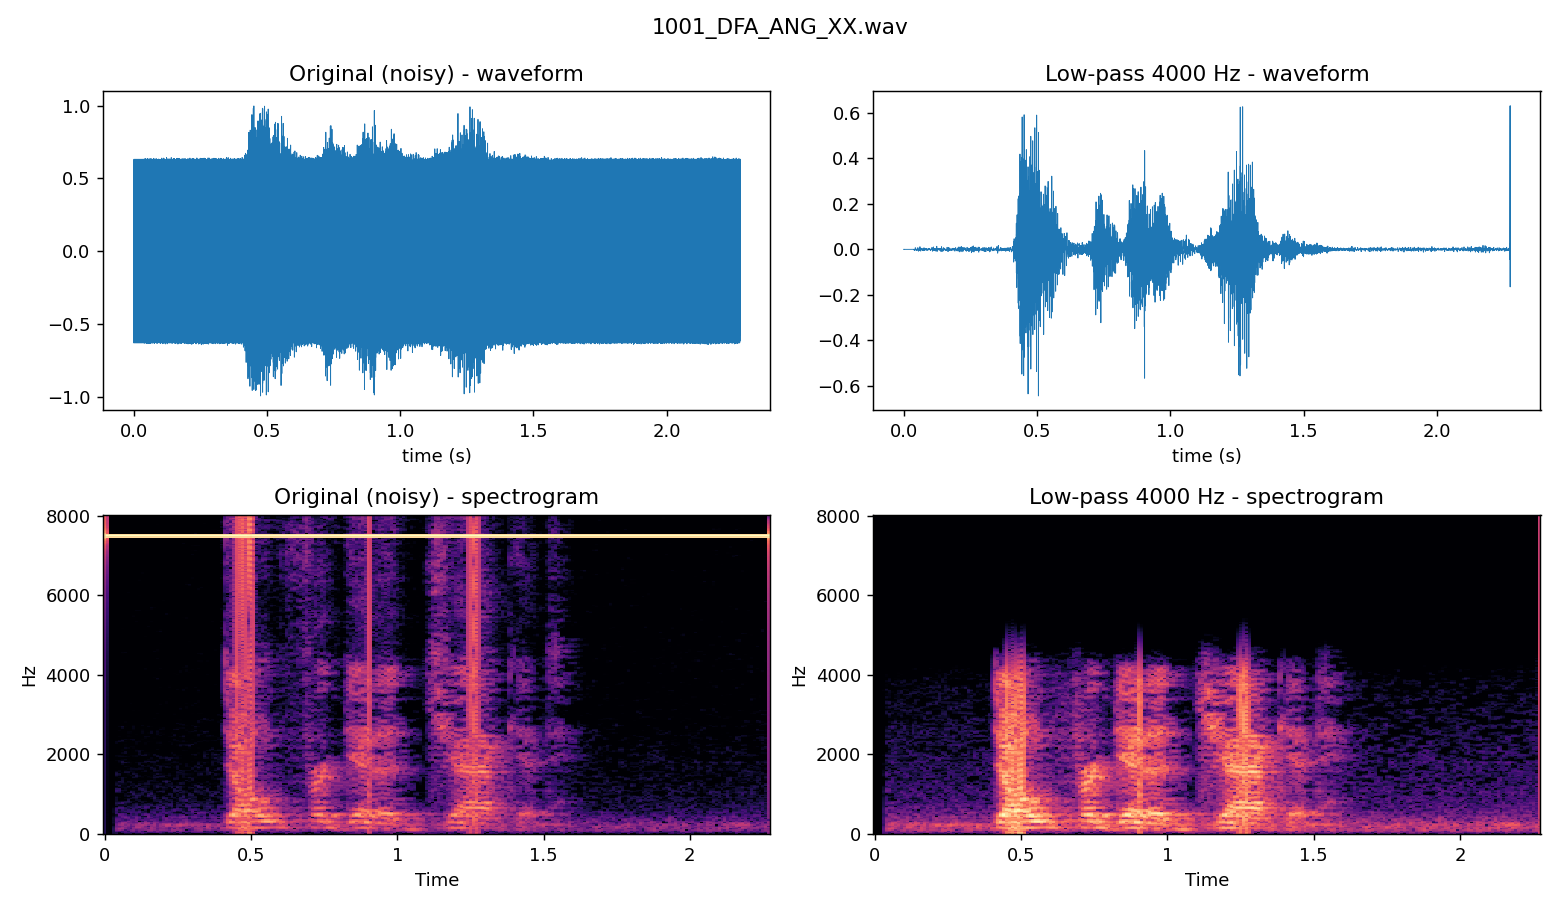
\includegraphics[width=0.95\textwidth]{q2_lowpass_demo.png}
  \caption{Effect of the 4\,kHz low-pass filter on a noisy clip: waveform (top) and
  spectrogram (bottom). Energy above 4\,kHz, which is mostly noise, is removed.}
  \label{fig:lowpass}
\end{figure}

\section{Feature extraction}\label{sec:q2feat}
\subsection{Literature review}
Speech emotion recognition traditionally relies on three families of hand-crafted
descriptors \cite{elayadi,schuller}:
\begin{itemize}
  \item \emph{spectral and cepstral} features describing vocal-tract shape and voice
        quality: MFCCs, mel-spectrogram, spectral centroid, bandwidth, contrast, roll-off
        and flatness;
  \item \emph{prosodic} features (fundamental frequency F0, energy, speaking rate), which
        capture arousal; anger and happiness, for instance, show higher and more variable
        pitch and energy than sadness;
  \item \emph{voice-quality and non-linear} features such as higher-order spectra.
        Bicoherence, the normalised bispectrum, measures quadratic phase coupling between
        frequency components and has been used for synthetic-speech detection and
        emotion analysis \cite{albadawy}.
\end{itemize}
The chromagram (12 pitch classes) suggested in the handout is mainly a music feature but
carries some intonation information, so it is included and evaluated.

\subsection{Implemented features}
Frame-level features use a 512-sample (32\,ms) window and a 160-sample (10\,ms) hop. They
are summarised over time by their mean and standard deviation, so every clip yields a
fixed-length vector of \textbf{242} values (Table~\ref{tab:q2feat}).

\begin{table}[H]
\centering
\caption{Audio feature groups (242 features per clip).}
\label{tab:q2feat}
\begin{tabularx}{\textwidth}{lcX}
\toprule
Group & Dim. & Description\\
\midrule
Fourier transform & 16 & log relative energy of the magnitude FFT in 16 equal bands from 0--4\,kHz\\
MFCC & 80 & 20 MFCCs and their deltas (mean, std)\\
Mel-spectrogram & 80 & 40 log-mel bands up to 4\,kHz (mean, std)\\
Chromagram & 24 & 12 pitch classes (mean, std)\\
Spectral shape & 22 & centroid, bandwidth, roll-off, flatness, 7-band spectral contrast (mean, std)\\
Prosody & 12 & F0 (YIN) mean, std, 10th/90th percentile and range over voiced frames; RMS energy mean, std and max; zero-crossing rate mean and std; voiced ratio; duration\\
Bicoherence & 8 & mean, variance, skewness, kurtosis of magnitude and phase of the segment-averaged bicoherence (256-sample segments, 64 frequency bins)\\
\bottomrule
\end{tabularx}
\end{table}

\noindent The bicoherence is estimated as
\begin{equation}
b(f_1,f_2)=\frac{\left|\mathbb{E}\left[X(f_1)X(f_2)X^*(f_1+f_2)\right]\right|}
{\sqrt{\mathbb{E}\left[|X(f_1)X(f_2)|^2\right]\,\mathbb{E}\left[|X(f_1+f_2)|^2\right]}},
\end{equation}
where the expectation is an average over Hann-windowed segments. Extraction of all 7,442
clips runs in parallel and takes about one minute.

\section{Classifiers and training protocol}\label{sec:q2clf}
Each classifier is wrapped in a pipeline with a \texttt{StandardScaler}, which is fitted on
the training data only:
\begin{itemize}
  \item \textbf{KNN}: $k\in\{3,\dots,31\}$, uniform or distance weights, Euclidean or cosine distance.
  \item \textbf{Logistic Regression} (multinomial, L2): $C\in\{0.001,\dots,10\}$.
  \item \textbf{Gaussian Naive Bayes}: variance smoothing $10^{-9}$ to $10^{-1}$.
  \item \textbf{SVM} with RBF kernel: $C\in\{0.3,\dots,30\}$, $\gamma\in\{\text{scale},10^{-3},3\cdot10^{-3},10^{-2}\}$.
  \item \textbf{Neural Network} (MLP, ReLU, Adam, early stopping): hidden layers
        (128), (256), (256,128), (512,256); L2 penalty $\alpha\in\{10^{-3},\dots,1\}$.
\end{itemize}
All grid points are trained on the training speakers and scored on the validation speakers.
The best setting is refit on training plus validation data and evaluated \emph{once} on the
14 unseen test speakers.

\section{Results}
\begin{table}[H]
\centering
\caption{Q2 emotion recognition on unseen speakers (6 classes, chance = 0.167).}
\label{tab:q2res}
\begin{tabular}{llccc}
\toprule
Model & Selected hyper-parameters & Val.\ acc. & \textbf{Test acc.} & Test macro-F1\\
\midrule
KNN & $k=15$, cosine, uniform & 0.469 & 0.408 & 0.381\\
Logistic Regression & $C=1$ & 0.525 & 0.519 & 0.519\\
Naive Bayes & smoothing $10^{-9}$ & 0.387 & 0.402 & 0.354\\
SVM (RBF) & $C=3$, $\gamma$=scale & 0.531 & \best{0.524} & \best{0.522}\\
Neural Network & (128), $\alpha=0.1$ & \best{0.537} & 0.513 & 0.513\\
\bottomrule
\end{tabular}
\end{table}

\begin{figure}[H]
  \centering
  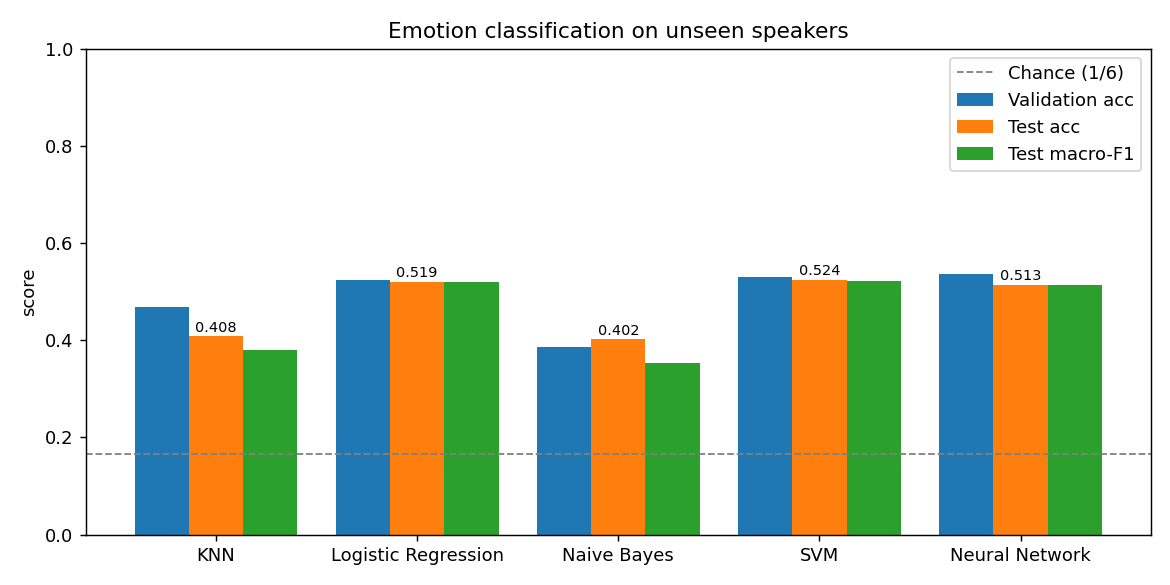
\includegraphics[width=0.8\textwidth]{q2_model_comparison.png}
  \caption{Validation accuracy, test accuracy and test macro-F1 of the five classifiers.}
\end{figure}

\begin{figure}[H]
  \centering
  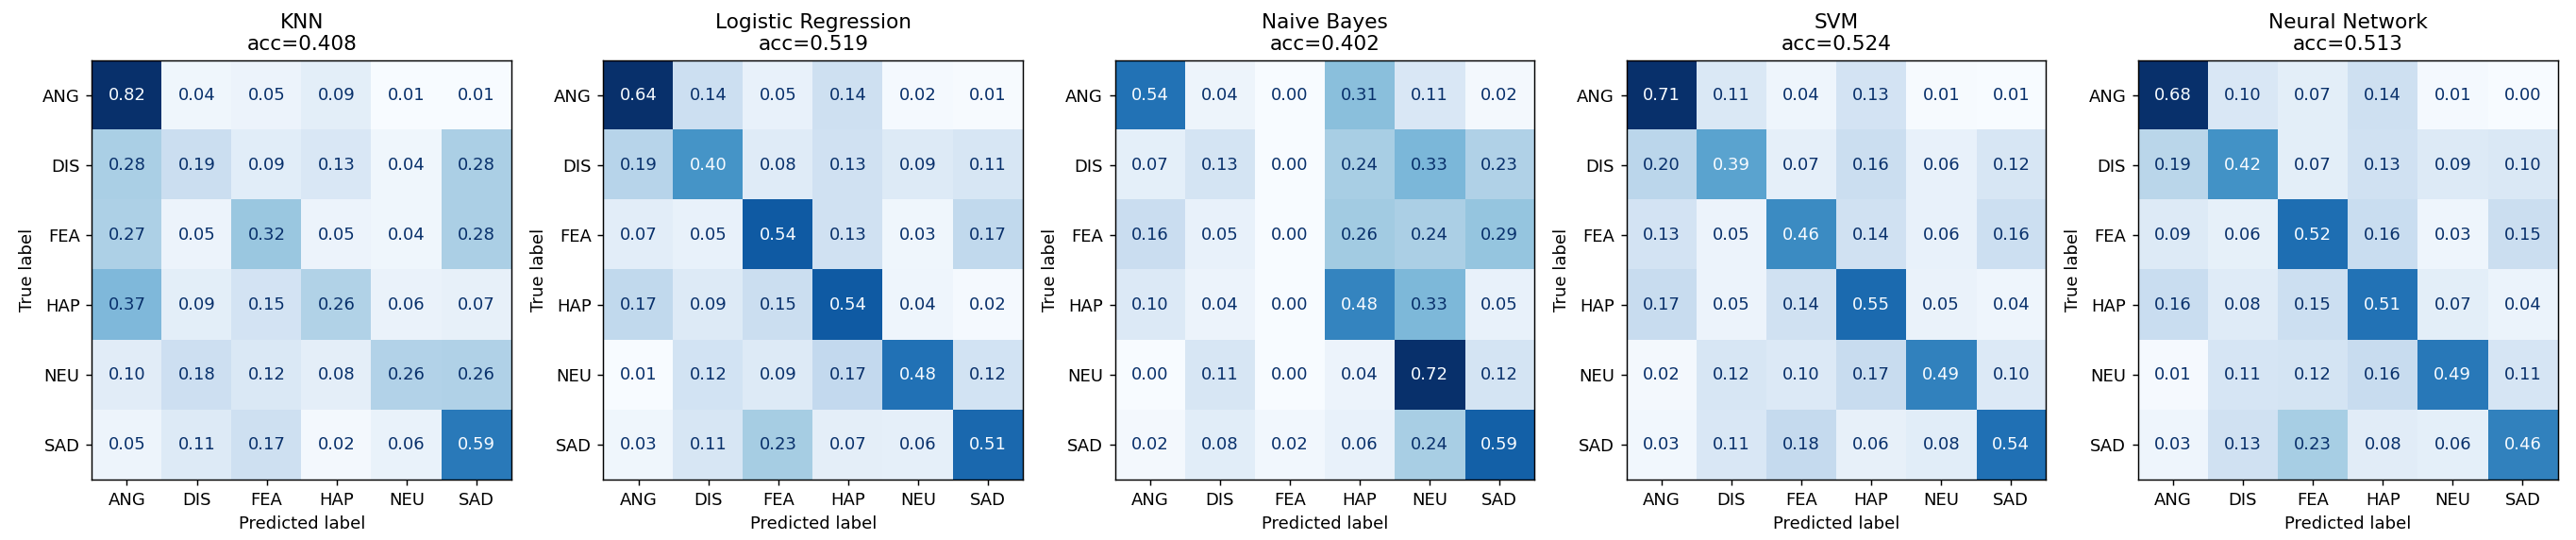
\includegraphics[width=\textwidth]{q2_confusion_matrices.png}
  \caption{Row-normalised test confusion matrices of the five classifiers.}
  \label{fig:q2cm}
\end{figure}

\paragraph{Discussion.}
The discriminative models (SVM, Logistic Regression, MLP) perform similarly at 51--52\%,
more than three times chance. This is in line with published speaker-independent
CREMA-D results that use hand-crafted features \cite{cremad}; human raters reach only
about 63\% on audio alone. Naive Bayes is weakest, because its independence assumption is
strongly violated (MFCC, mel and spectral features are highly correlated). KNN suffers
from the high dimensionality and from speaker differences dominating the distances.
Per class (SVM), \emph{Anger} is recognised best (F1 = 0.63, recall 0.71) and
\emph{Disgust} worst (F1 = 0.44). The main confusions in Figure~\ref{fig:q2cm} are
Disgust$\leftrightarrow$Anger, Fear$\leftrightarrow$Sad and Happy$\leftrightarrow$Anger.
These are emotions that share arousal (Anger and Happy are both high) or valence, which
acoustic features capture poorly. Although the MLP had the highest validation accuracy and
is therefore saved as the deployed model, the SVM generalised slightly better to the test
speakers. The difference (1.1 points, about 13 clips) is within the variation expected
from 14 test speakers.

\section{Further analysis}
\subsection{Feature-group ablation}
Using the selected SVM, each feature group was evaluated alone, and the full set was
evaluated with each group left out (Table~\ref{tab:abl}).
\begin{table}[H]
\centering
\caption{Feature ablation (SVM, test accuracy).}
\label{tab:abl}
\begin{tabular}{lccc}
\toprule
Group & Dim. & Group alone & All \emph{minus} group\\
\midrule
FFT bands & 16 & 0.383 & 0.525\\
MFCC & 80 & \best{0.490} & \best{0.504}\\
Mel-spectrogram & 80 & 0.456 & 0.527\\
Chromagram & 24 & 0.351 & 0.525\\
Spectral shape & 22 & 0.419 & 0.520\\
Prosody & 12 & 0.449 & 0.515\\
Bicoherence & 8 & 0.289 & 0.524\\
\midrule
All features & 242 & \multicolumn{2}{c}{0.524}\\
\bottomrule
\end{tabular}
\end{table}
\noindent MFCCs are the most informative group: they are the best on their own, and
removing them causes the largest drop. With only 12 values, prosody is remarkably strong
(0.449), which confirms that pitch and energy carry emotional arousal. Bicoherence and
chroma are weak on their own and redundant given the other groups.

\subsection{Choice of the low-pass cut-off}
\begin{table}[H]
\centering
\caption{Effect of the low-pass cut-off frequency (SVM, test accuracy).}
\begin{tabular}{lccccc}
\toprule
Cut-off & 2\,kHz & 3\,kHz & 4\,kHz & 6\,kHz & none ($\approx$8\,kHz)\\
\midrule
Test accuracy & 0.526 & 0.531 & 0.524 & 0.529 & 0.529\\
\bottomrule
\end{tabular}
\end{table}
\noindent Accuracy hardly changes between 2\,kHz and no filtering, because the features are
computed in the 0--4\,kHz band. The emotional information is concentrated in the low
frequencies, so the filter removes noise without losing useful signal. 4\,kHz is kept as a
conservative choice that preserves the full telephone speech band.

\subsection{Ensemble and per-speaker normalisation}
\begin{table}[H]
\centering
\caption{Ensemble and speaker normalisation (test accuracy / macro-F1).}
\label{tab:extras}
\begin{tabular}{lcc}
\toprule
Model & Global scaling & Per-speaker normalisation\\
\midrule
SVM & 0.524 / 0.522 & \best{0.613} / 0.611\\
Logistic Regression & 0.519 / 0.519 & 0.609 / 0.608\\
Neural Network & 0.513 / 0.513 & 0.589 / 0.589\\
Soft-voting ensemble (SVM+LR+NN) & 0.538 / 0.537 & \best{0.613} / \best{0.612}\\
\bottomrule
\end{tabular}
\end{table}
\noindent A soft-voting ensemble of the three strongest models improves the result to
53.8\%. A much larger gain comes from \textbf{per-speaker normalisation}: every feature is
z-scored using the mean and standard deviation of all clips of the \emph{same speaker}. This
removes speaker-specific characteristics (average pitch, timbre, recording level) and keeps
the emotion-related deviations, raising test accuracy by about 9 points to
\textbf{61.3\%}. The technique needs several recordings of a speaker but \emph{no labels},
so it is legitimate in practice, e.g.\ for a call-centre agent or a returning user. Accuracy
also depends on emotion intensity: clips with low intensity are hardest (35.7\%), and
medium and high intensity reach 51.4\%.

\section{Limitations}
Accuracy is limited by acted, short and noisy utterances and by genuine ambiguity between
emotions. Even human raters disagree on many CREMA-D clips. Deep representations
(CNNs on log-mel spectrograms or pre-trained wav2vec-style encoders) would be the next step
beyond the classical features required here.

% ===================================================================== Q3
\chapter{Q3: Surface Defect Detection and Classification}

\section{Problem statement}
The aim is to detect defects in images of a paper reel. This involves (i) classifying each
image into one of three classes (defect-free paper, paper with a hole, paper with a pen
mark) using a classical feature pipeline and four classifiers (SVM, Naive Bayes, Logistic
Regression, Neural Network), and (ii) localising the defect with a bounding box in
defective images.

\section{Dataset analysis}
The dataset (downloaded from the Google Drive folder in the handout) contains
\textbf{1,500} JPEG images of 2000$\times$2000 pixels: 509 \emph{paper}, 489 \emph{hole}
and 502 \emph{penMark}. Analysis of the data showed several properties that shaped the
design:
\begin{itemize}
  \item The three colour channels are identical, so the images are effectively
        \textbf{grayscale}, and a ``colour histogram'' is an intensity histogram.
  \item The defects are \textbf{tiny}: a hole is a dark speck of about 5--25\,px (less than
        0.01\% of the image) and a pen mark is a thin dark stroke of about 15--120\,px. By
        contrast, the paper texture and a strong \textbf{illumination gradient} dominate the
        image (Figure~\ref{fig:q3pipe}, left). Global features of the raw image therefore
        see mostly lighting and texture.
  \item A few faint dark blemishes appear at the \textbf{same position in every image}
        (dust on the lens or background). A detector must learn to ignore them.
  \item Image numbers 0--1499 are shared across the classes and interleaved randomly, so
        the images are not ordered video frames and a stratified random split is
        appropriate.
\end{itemize}
The images are split with stratification into 1,050 training, 225 validation and 225 test
images (70/15/15).

\section{Pre-processing and candidate regions}
\begin{enumerate}
  \item \textbf{Down-sampling} to 1000$\times$1000 with area interpolation, which preserves
        small dark spots.
  \item \textbf{Illumination flattening.} The background is estimated with a wide Gaussian
        blur ($\sigma=20$\,px) and subtracted, giving the residual $r = I - G_\sigma * I$.
  \item \textbf{Robust z-score map} $z = (r-\operatorname{median}(r))/(1.4826\,\mathrm{MAD}(r))$.
        Clean paper texture stays within about $[-7,+10]$, while holes and ink reach $-10$ to
        $-50$, independently of the lighting.
  \item \textbf{Candidate proposals.} Pixels with $z<-4$ (after light smoothing) are
        thresholded, a 7$\times$7 morphological closing joins the broken strokes of a pen
        mark, and connected components are ranked by their ``darkness mass''
        $\sum(-z)$. The top proposals are passed on.
\end{enumerate}
A calibration over all 1,500 images confirmed that the method separates the classes well:
the darkest response on clean paper is $-5.9\pm0.6\sigma$, compared with
$-30.7\pm10.5\sigma$ for holes and $-23.8\pm4.3\sigma$ for pen marks. Pen-mark regions are
about 4--5 times larger than hole regions.

\begin{figure}[H]
  \centering
  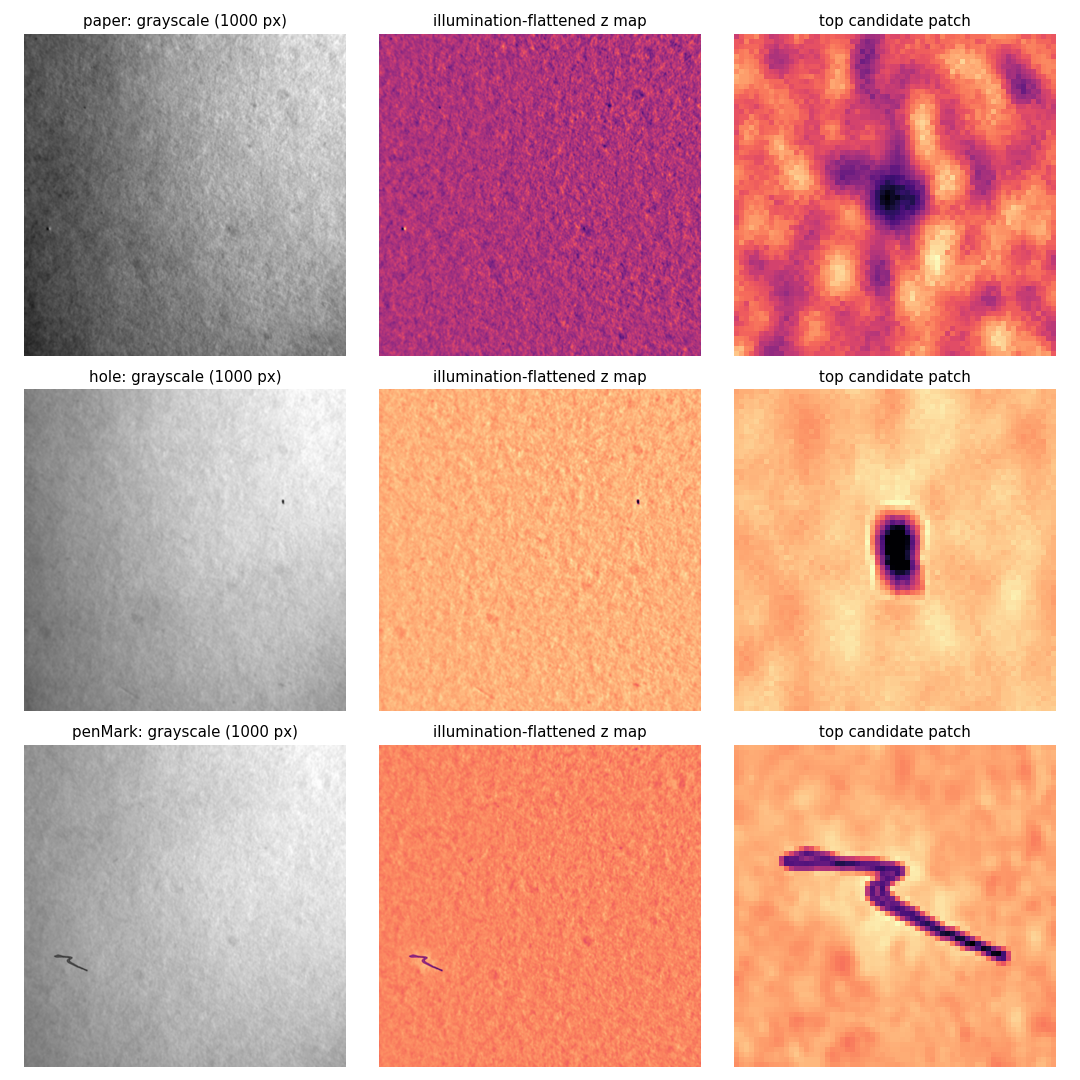
\includegraphics[width=0.8\textwidth]{q3_preprocessing_pipeline.png}
  \caption{Pre-processing for a test image of each class: grayscale input,
  illumination-flattened z-map, and the patch around the top candidate.}
  \label{fig:q3pipe}
\end{figure}

\section{Feature extraction}\label{sec:q3feat}
\subsection{Literature review}
Classical surface-inspection systems describe defects by intensity statistics, texture and
shape \cite{xie,neogi}. Besides the features in the handout (colour histogram, spatial
binning \cite{udacity}, HOG \cite{hog}), we used:
\begin{itemize}
  \item \textbf{Local Binary Patterns (LBP)} \cite{lbp}, a grey-scale-invariant texture
        descriptor widely used for surface and fabric defect detection;
  \item \textbf{Grey-Level Co-occurrence Matrix (GLCM)} statistics \cite{haralick}
        (contrast, dissimilarity, homogeneity, energy, correlation), the classical texture
        features for steel, wood and paper inspection;
  \item \textbf{shape descriptors} of the segmented blob (area, bounding-box aspect ratio,
        extent, solidity, eccentricity, major and minor axis, circularity, Hu moment
        invariants \cite{hu}), which directly encode ``compact spot'' versus ``elongated
        stroke''.
\end{itemize}

\subsection{Implemented features}
\begin{table}[H]
\centering
\caption{Image feature groups (4,959 features in total).}
\label{tab:q3feat}
\begin{tabularx}{\textwidth}{llcX}
\toprule
Set & Group & Dim. & Description\\
\midrule
\multirow{4}{*}{Global}
 & Colour histogram & 32 & intensity histogram of the image\\
 & z histogram & 32 & log-count histogram of the z-map\\
 & Spatial binning & 1,024 & z-map min-pooled to 32$\times$32\\
 & HOG & 1,764 & HOG of the z-map (128$\times$128, 16\,px cells, 2$\times$2 blocks, 9 bins)\\
\midrule
\multirow{6}{*}{Patch}
 & z histogram & 16 & histogram of the candidate patch\\
 & Spatial binning & 256 & patch resized to 16$\times$16\\
 & HOG & 1,764 & patch 64$\times$64, 8\,px cells, 2$\times$2 blocks, 9 bins\\
 & LBP & 10 & uniform LBP ($P=8,R=1$) histogram\\
 & GLCM & 40 & 5 properties $\times$ 2 distances $\times$ 4 angles\\
 & Shape & 21 & blob geometry, darkness statistics, 7 Hu moments, patch scale\\
\bottomrule
\end{tabularx}
\end{table}
\noindent The patch is a square crop centred on the candidate, with a side of
$\max(64, 1.4\times$ the blob size$)$, resized to 64$\times$64. This keeps the whole pen
stroke inside the patch.

\paragraph{Data augmentation.} Paper has no preferred orientation, so every training and
validation image is also used rotated by 90$^\circ$ and 180$^\circ$ and flipped
horizontally ($\times$4 data). Test images are never augmented.

\section{Task (i): three-class classification}\label{sec:q3cls}
All classifiers use a \texttt{StandardScaler}, a validation grid search
(SVM: $C$, $\gamma$; Naive Bayes: smoothing; Logistic Regression: $C$; MLP: architecture and
$\alpha$), refitting on augmented training plus validation data, and a single evaluation on
the 225 test images. Three feature sets were compared to measure the value of the candidate
patch.

\begin{table}[H]
\centering
\caption{Q3 three-class test accuracy (225 test images) for each feature set. Validation accuracy in parentheses.}
\label{tab:q3res}
\begin{tabular}{lccc}
\toprule
Classifier & Global (2,852) & Patch (2,107) & All (4,959)\\
\midrule
SVM (RBF) & 0.969 (0.973) & 0.982 (\best{0.991}) & 0.987 (0.987)\\
Naive Bayes & 0.942 (0.920) & 0.960 (0.960) & 0.987 (0.964)\\
Logistic Regression & 0.978 (0.973) & 0.978 (0.973) & \best{0.991} (0.982)\\
Neural Network (MLP) & 0.982 (0.969) & 0.973 (0.982) & 0.987 (0.978)\\
\bottomrule
\end{tabular}
\end{table}

\begin{figure}[H]
  \centering
  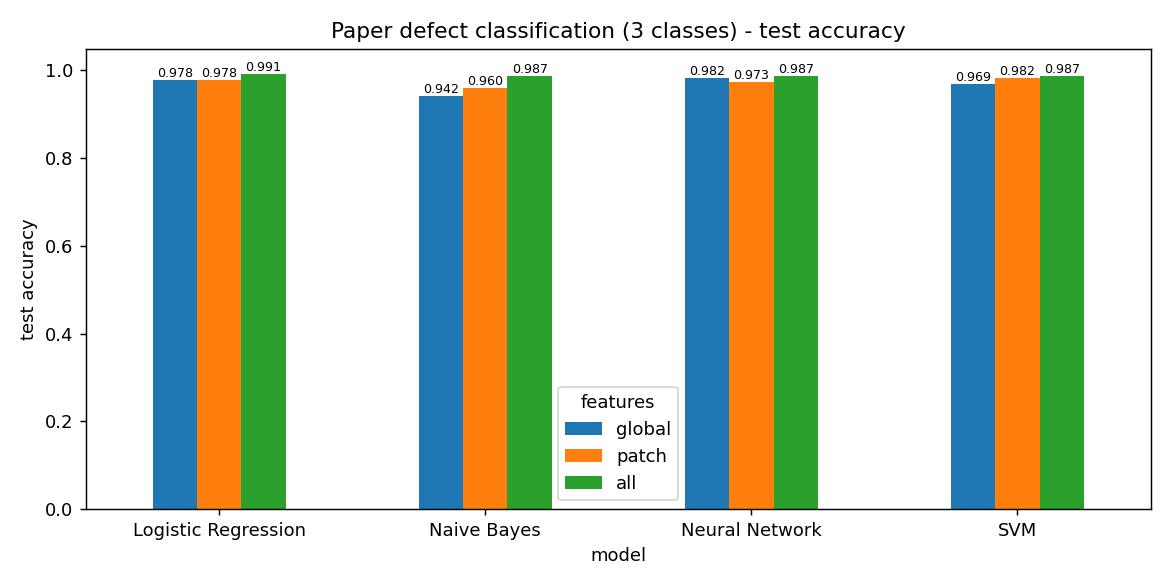
\includegraphics[width=0.8\textwidth]{q3_model_comparison.png}
  \caption{Test accuracy of the four classifiers for each feature set.}
\end{figure}

\begin{figure}[H]
  \centering
  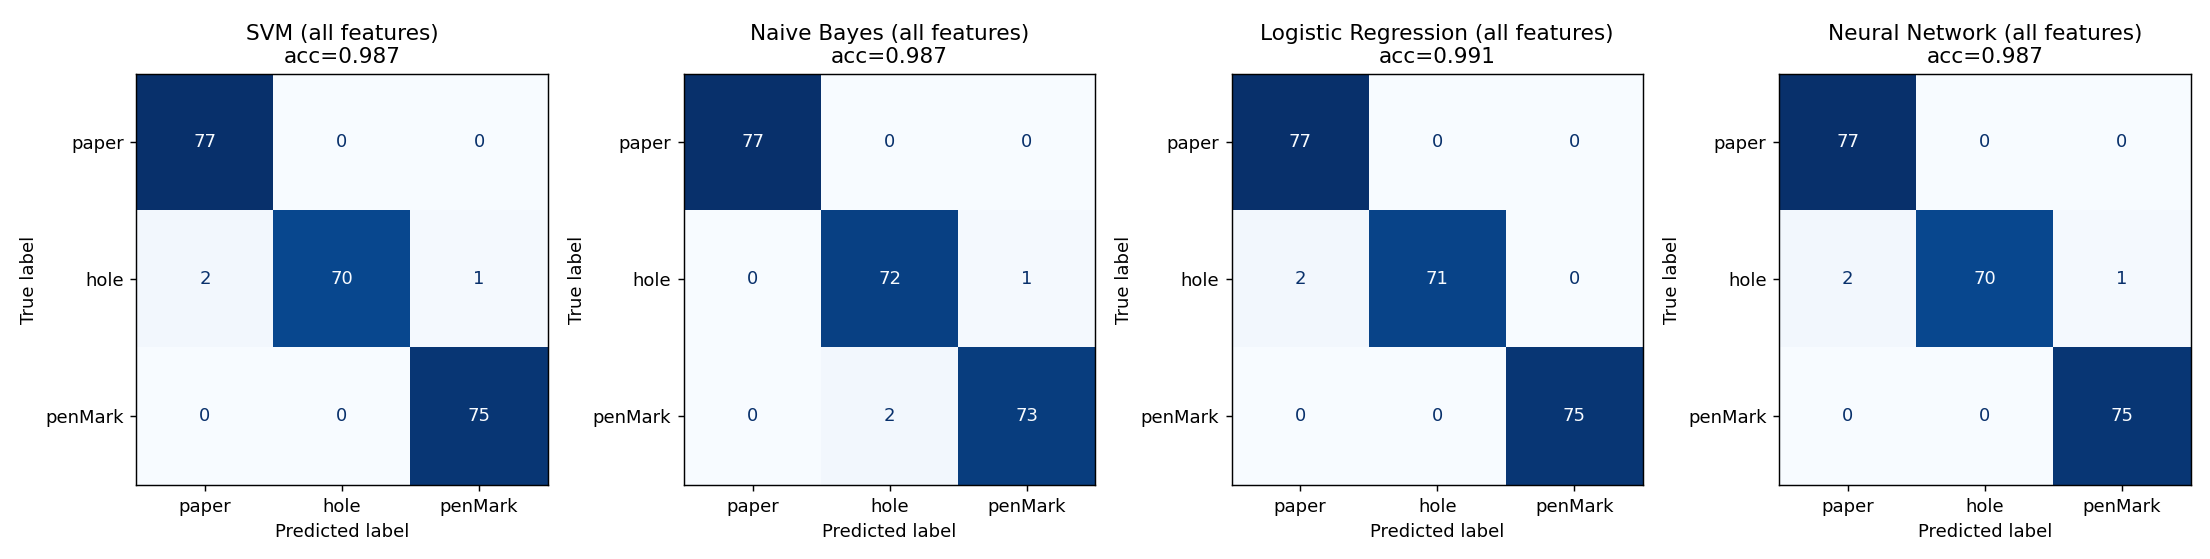
\includegraphics[width=\textwidth]{q3_confusion_matrices.png}
  \caption{Test confusion matrices with all features.}
\end{figure}

\paragraph{Discussion.}
All four classifiers perform very well (94--99\%) \emph{because} the pre-processing makes
the defects visible: on the illumination-flattened z-map, even the global HOG and
spatial-binning features carry the defect signal. The candidate-patch features
(texture and shape of the isolated object) give the highest validation accuracy, and
combining both sets gives the best test accuracy (98.7--99.1\%). With all features even
Naive Bayes reaches 98.7\%, which shows that the shape descriptors make the classes nearly
linearly separable. The few remaining errors are almost all holes: very faint or very small
holes that look like paper texture, and elongated holes that look like a short pen stroke
(Figure~\ref{fig:q3err}).

\section{Task (ii): defect localisation}\label{sec:q3loc}
\subsection{Method}
Localisation reuses the trained classifiers. A \textbf{region classifier} is trained on the
patch features of the \emph{top five} proposals of every training image:
\begin{itemize}
  \item the top proposal of a hole or pen-mark image is labelled with the image class;
  \item all proposals of defect-free images, and the lower-ranked proposals of defect images
        (mostly the static lens blemishes and texture specks), are labelled
        \emph{background}. These act as \textbf{hard negatives} (5,235 training proposals:
        694 defects, 4,541 background).
\end{itemize}
At inference, every proposal is scored, and the proposal with the highest $P(\text{defect})$
is the detected defect. Its connected-component bounding box, scaled back to the
2000$\times$2000 image, is drawn with the predicted class and confidence. The same decision
also gives an image-level class (\emph{multi-proposal} decision). The four classifier
families were tuned for this task by image-level validation accuracy
(Table~\ref{tab:region}).

A first version trained the region classifier only on top proposals. It was rejected after
analysis because it labelled faint background specks on clean paper as holes: it had never
seen such regions during training. The hard-negative training fixes this.

\begin{table}[H]
\centering
\caption{Region classifier (multi-proposal decision) accuracy.}
\label{tab:region}
\begin{tabular}{lcc}
\toprule
Classifier & Val.\ acc. & Test acc.\\
\midrule
SVM (RBF, $C=10$, $\gamma=10^{-4}$) & \best{0.996} & \best{0.973}\\
Naive Bayes & 0.969 & 0.969\\
Logistic Regression ($C=0.01$) & 0.987 & 0.964\\
Neural Network (256,64) & 0.991 & 0.973\\
\bottomrule
\end{tabular}
\end{table}

\noindent Because the multi-proposal SVM had the highest validation accuracy of all models
(0.996), it was selected as the final model for both tasks. On the test set it recognises
all 77 clean images correctly (no false alarms), 68 of 73 holes and 74 of 75 pen marks,
giving 97.3\% overall. The single-candidate classifiers of Table~\ref{tab:q3res} are
slightly better on test (up to 99.1\%); the difference is 4 images and is within the noise
of a 225-image test set.

\subsection{Localisation results}
No ground-truth boxes are provided, so localisation was evaluated in two ways:
\begin{itemize}
  \item \textbf{Consistency.} For 146 of the 148 defective test images, the chosen proposal
        is also the darkest region of the image. In the other two, the region classifier
        correctly passed over a static blemish.
  \item \textbf{Visual inspection} of zoomed crops (Figure~\ref{fig:q3loc}) and of all
        misclassified images (Figure~\ref{fig:q3err}). In every inspected case the box lies
        tightly on the real hole or pen mark, including the 6 images whose class was wrong.
        Pen-mark boxes cover the whole stroke, because the morphological closing merges its
        fragments.
\end{itemize}

\begin{figure}[H]
  \centering
  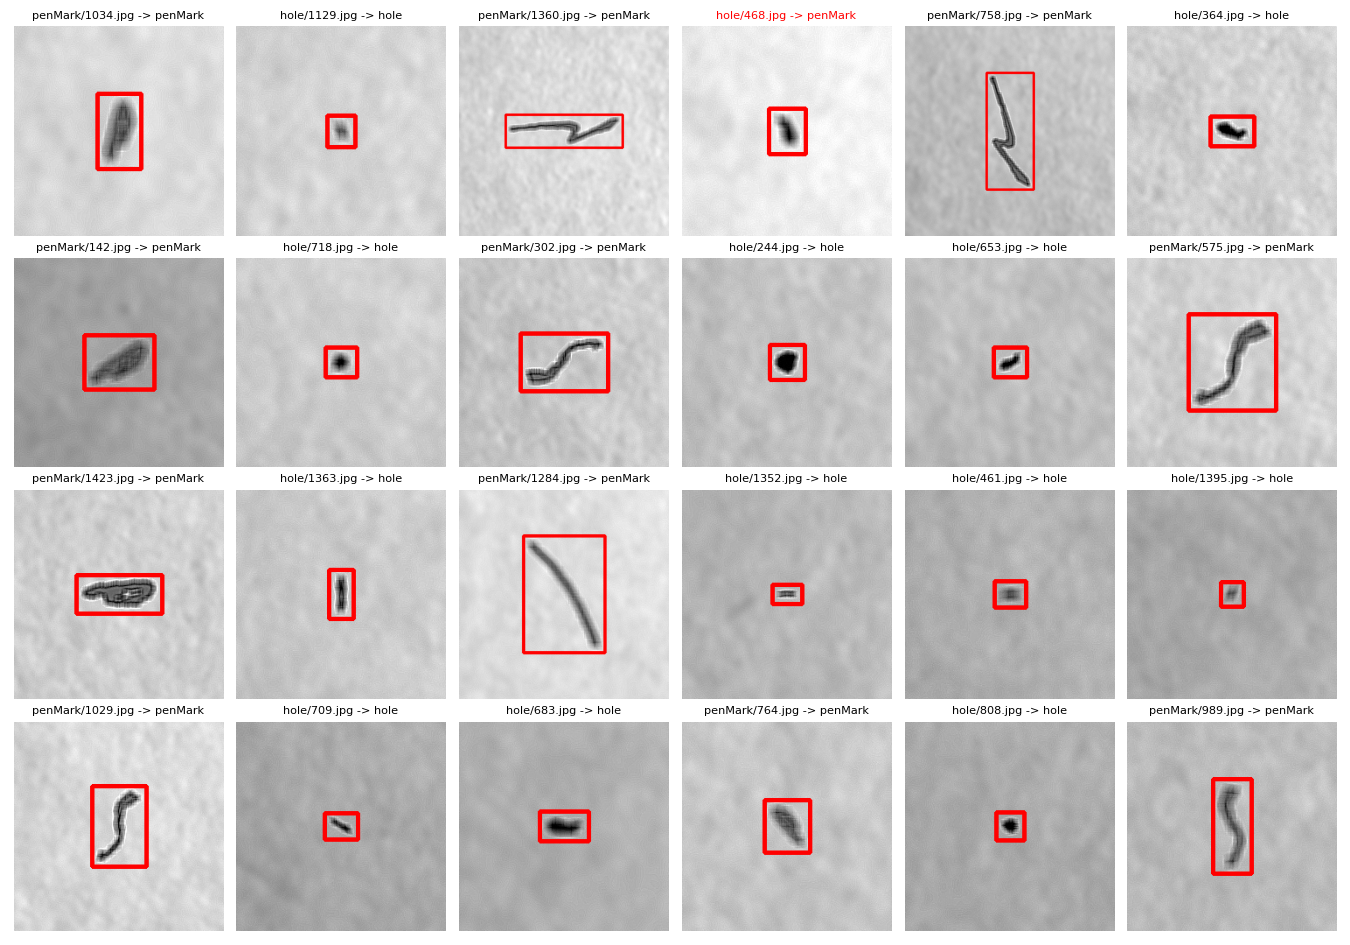
\includegraphics[width=\textwidth]{q3_localization_zoom.png}
  \caption{Detected bounding boxes on 24 random defective test images (zoomed on the box;
  titles show the true class and the prediction; red = wrong class).}
  \label{fig:q3loc}
\end{figure}

\begin{figure}[H]
  \centering
  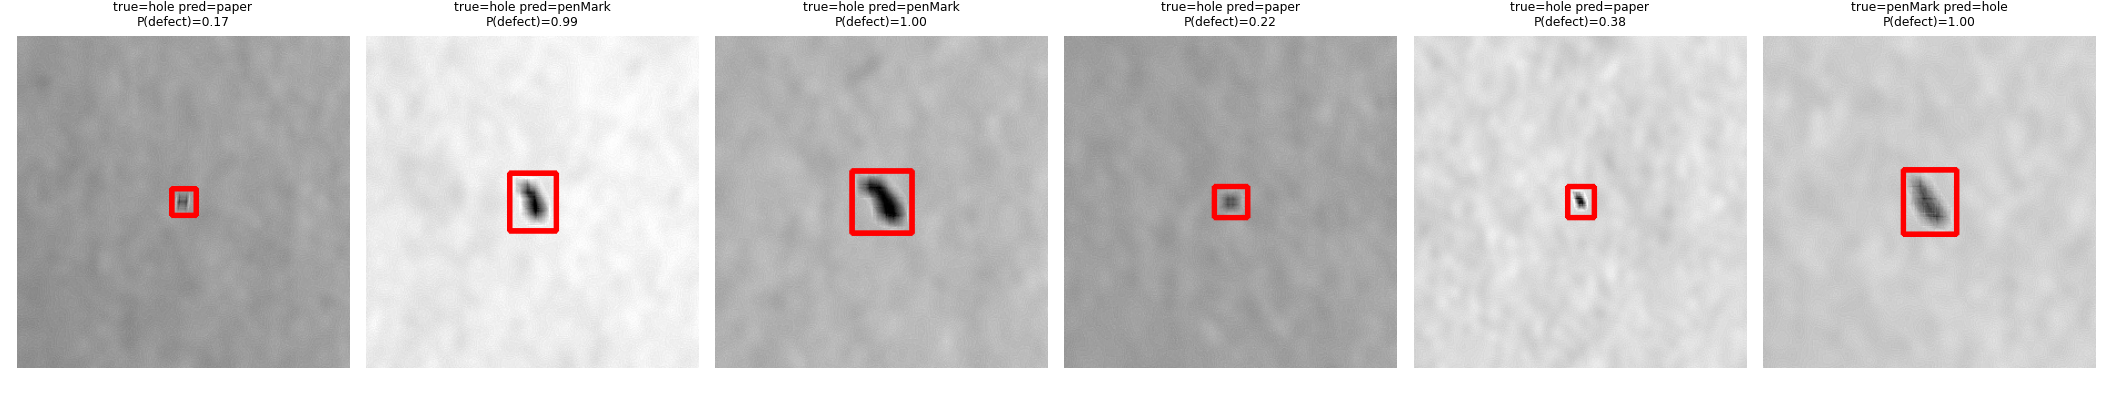
\includegraphics[width=\textwidth]{q3_errors.png}
  \caption{All misclassified test images. Each box is still on the defect; the errors are
  faint holes (predicted paper) and elongated holes resembling pen strokes.}
  \label{fig:q3err}
\end{figure}

\section{Limitations}
The method assumes a single dominant dark defect per image and dark defects on light paper.
Bright defects (for example tears with back-lighting) would need a symmetric
threshold. A quantitative IoU evaluation would require manually annotated boxes. Detecting
very faint holes is the main remaining error source; higher-resolution processing around
proposals could reduce it.

% ============================================================== usability
\chapter{Software Design and Ease of Use}

\section{Organisation of the code}
Each question has a clear separation of concerns:
\begin{itemize}
  \item a \emph{feature module} (\texttt{audio\_features.py}, \texttt{defect\_features.py})
        with pure functions for pre-processing and feature extraction, documented with
        docstrings;
  \item a \emph{training script} that runs the whole experiment (split, features, tuning,
        evaluation, figures, model export) with one command;
  \item a \emph{prediction script} (\texttt{predict.py}) that applies the saved model to new
        files.
\end{itemize}
All results (CSV tables, classification reports, figures, tuning logs) are written to each
question's \texttt{results/} folder, and models are saved with \texttt{joblib} to
\texttt{models/}.

\section{How to run}
\begin{lstlisting}
pip install -r requirements.txt
python q1/q1_knn.py
python q2/q2_audio_sentiment.py --cutoff-study
python q2/q2_extras.py
python q3/q3_defect_detection.py
python q2/predict.py some_clip.wav
python q3/predict.py some_image.jpg        # writes annotated image to q3/predictions/
streamlit run app.py                       # interactive web demo
\end{lstlisting}

\section{Interactive web application}
\texttt{app.py} provides a browser interface to all three models. It accepts typed
headlines, microphone recordings, uploaded WAV files and uploaded images, as well as
examples from the test sets. Chapter~\ref{ch:innov} describes it in detail.

\section{Public repository}
The complete project (code, trained models, results, report) is published at
\url{https://github.com/hbnasir23/ml-cep-ct317}. The audio and image datasets are not stored in the repository because
of their size (1.2\,GB and 1.6\,GB); the README explains how to download them.

\section{Reproducibility}
Seeds are fixed (42), the expensive feature extraction is cached in \texttt{cache/}, and
every number in this report is produced by the scripts. Two full runs of the Q3 pipeline
gave identical results.


% ============================================================ innovation
\chapter{Innovation: An Explainable Interactive Application}
\label{ch:innov}
Beyond the required experiments, the project contributes an \textbf{interactive,
explainable front-end}. Anyone can test the trained models with their own input, and each
prediction comes with the evidence behind it. It is started with
\texttt{streamlit run app.py} and has one tab per question.

\section{Q1: explain a headline by its neighbours}
The user types any headline. The app shows the predicted label, $P(\text{real})$ and how
many of its words the model knows. Because KNN is an instance-based learner, the prediction
can be explained \emph{exactly}: the app lists the $k=12$ nearest training headlines with
their cosine distances and labels (Figure~\ref{fig:appq1}). This makes the effect of the
cosine metric visible: neighbours share the same words regardless of length.
\begin{figure}[H]
\centering
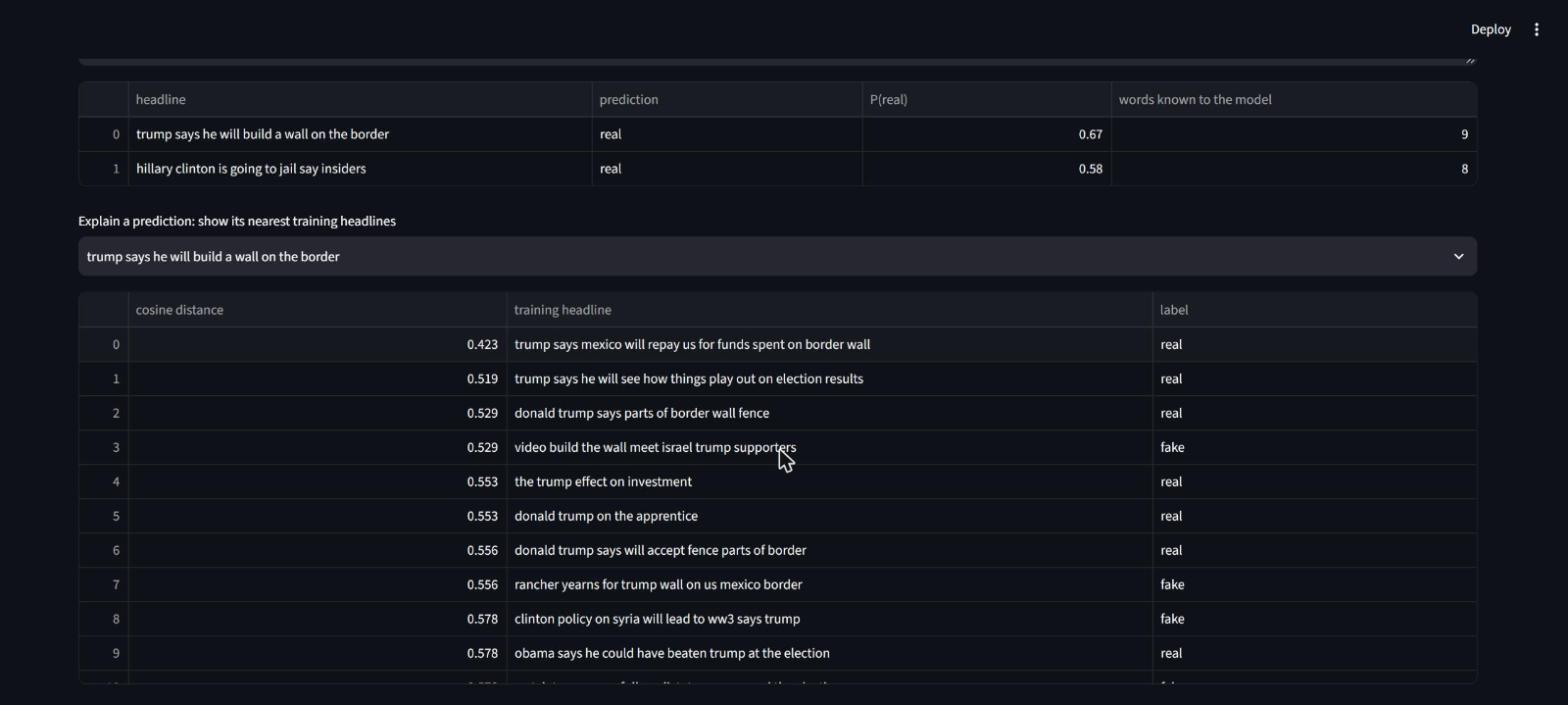
\includegraphics[width=\textwidth]{app_q1.jpg}
\caption{Q1 tab: prediction for user headlines and the 12 nearest training headlines that
explain it.}
\label{fig:appq1}
\end{figure}

\section{Q2: live microphone input and ``what the filter removed''}
The user can \textbf{record their own voice in the browser}, upload a WAV file, or replay a
clip from the unseen test speakers. The app shows the predicted emotion, the full
probability distribution, and the spectrogram before and after the 4\,kHz low-pass filter.
Figure~\ref{fig:appq2} is an instructive case: the noisy recording contains a constant
tone at about 7.5\,kHz, which the filter removes completely. The model hesitates between
\emph{Happy} (0.45) and the true \emph{Anger} (0.43), two high-arousal emotions it often
confuses.
\begin{figure}[H]
\centering

\includegraphics[width=0.85\textwidth]{app_q2_mic.jpg}
\par\medskip
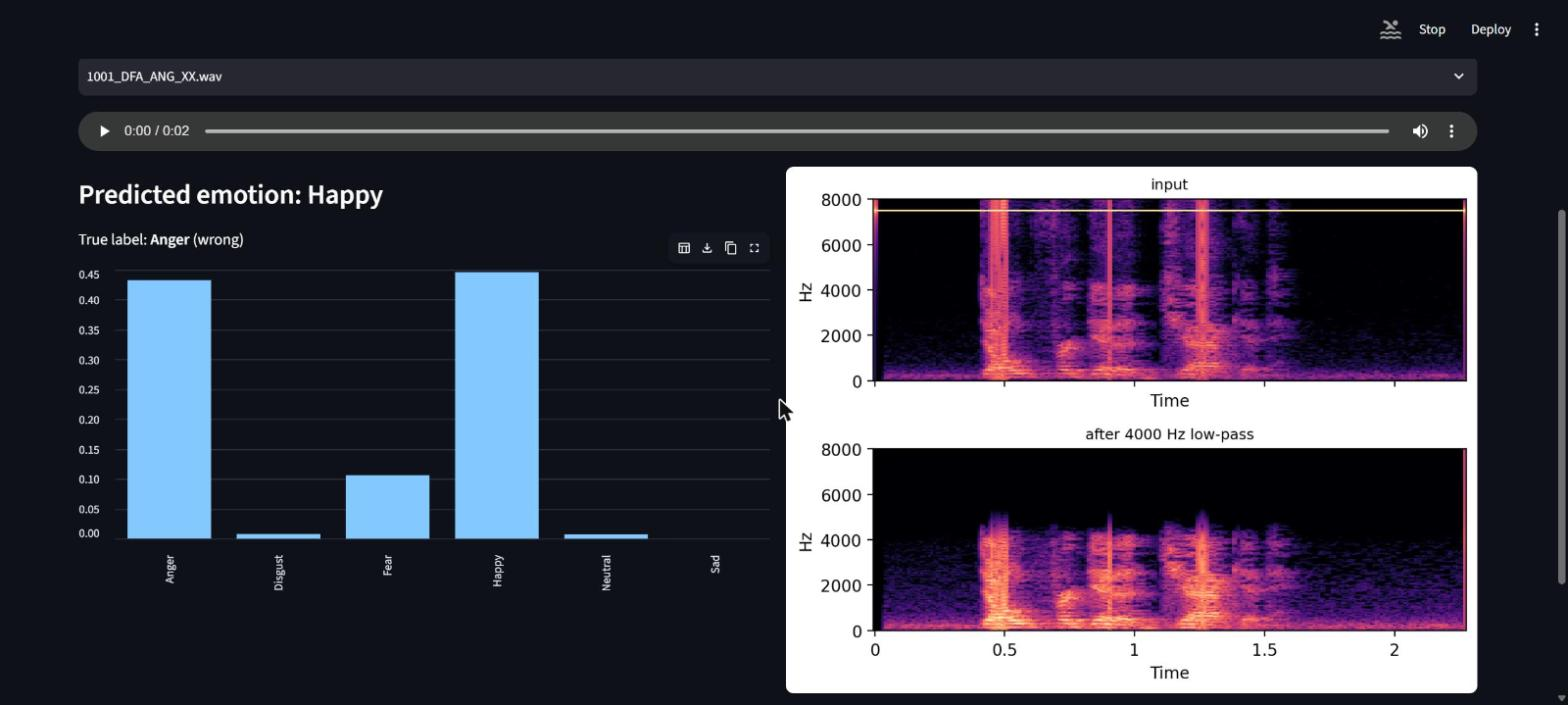
\includegraphics[width=0.85\textwidth]{app_q2.jpg}
\caption{Q2 tab: microphone recording (top); prediction, probabilities and the spectrogram
before and after filtering (bottom).}
\label{fig:appq2}
\end{figure}

\section{Q3: defect localisation with a look inside the pipeline}
The user uploads a paper image or picks a test image. The app shows the class, its
probabilities, the bounding box in original pixel coordinates and a zoom on the defect. An
expandable panel shows \emph{how the model sees the image}: the illumination-flattened z-map
with all five candidate regions and, for every candidate, its darkness score, size and
class probabilities from the region classifier (Figure~\ref{fig:appq3}). This makes it clear
why a faint speck is rejected while the pen stroke is accepted.
\begin{figure}[H]
\centering
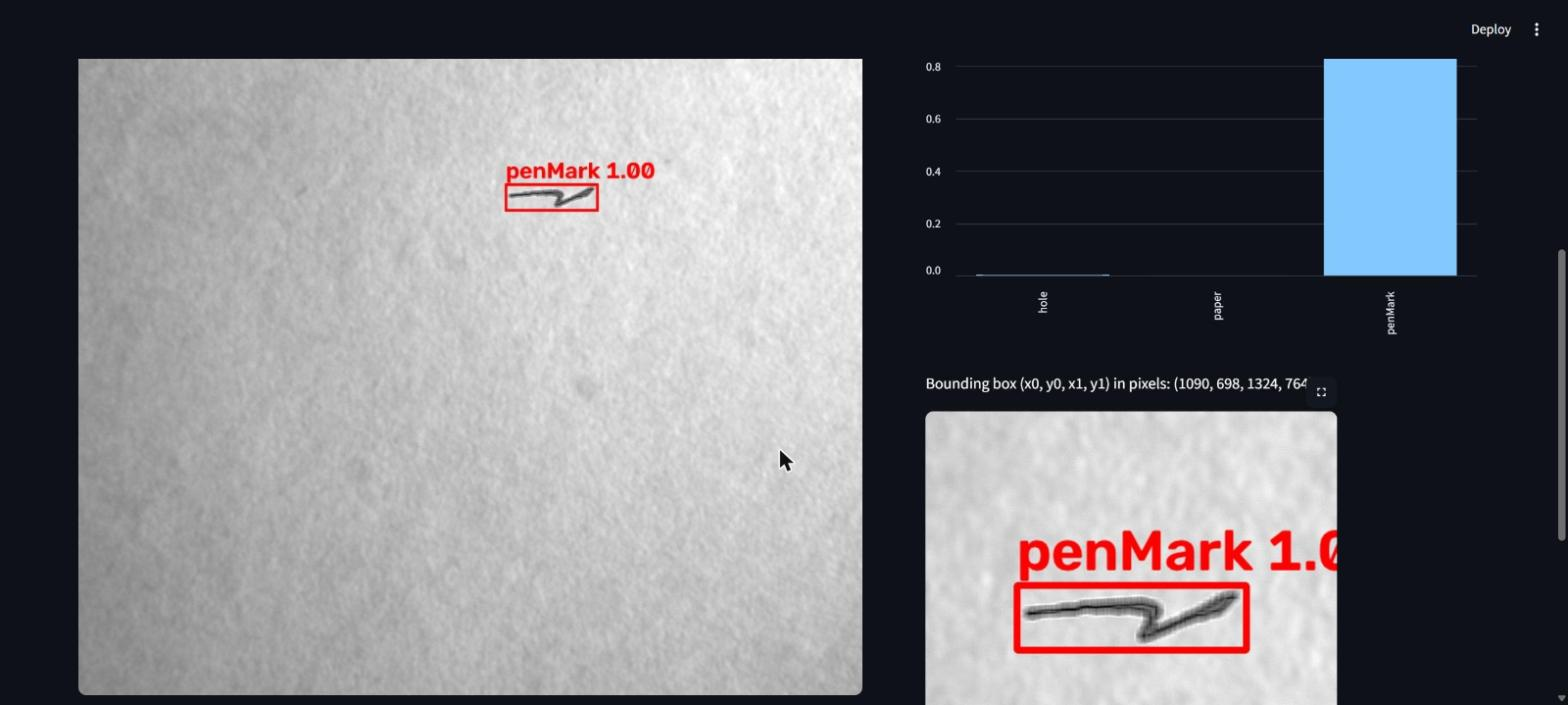
\includegraphics[width=0.85\textwidth]{app_q3.jpg}
\par\medskip
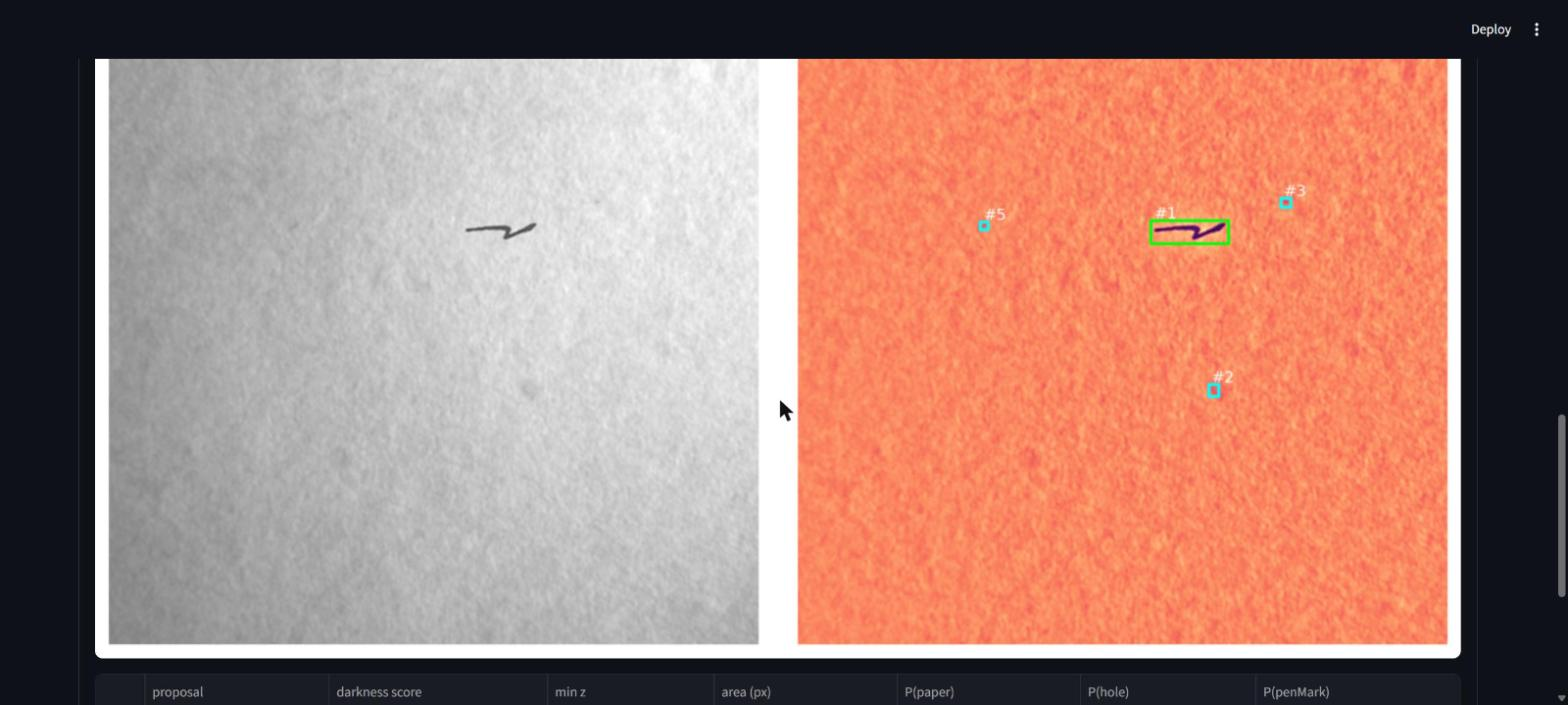
\includegraphics[width=0.85\textwidth]{app_q3_zmap.jpg}
\caption{Q3 tab: detected pen mark with bounding box and zoom (top); z-map with the five
scored proposals, where \#1 (green) is the selected defect (bottom).}
\label{fig:appq3}
\end{figure}

\section{Methodological innovations}
\begin{itemize}
  \item \textbf{Speaker-independent evaluation and per-speaker normalisation (Q2).} Most
        simple tutorials split clips at random and report inflated accuracies. We evaluate
        on unseen voices and show that label-free per-speaker normalisation adds about 9
        points (52.4\%$\rightarrow$61.3\%).
  \item \textbf{Proposal-based classical detector with hard negatives (Q3).} Instead of
        describing the whole image, the pipeline isolates candidate objects (illumination
        flattening, robust z-score, morphology) and learns to reject static lens blemishes.
        The same classifier performs both classification and localisation.
  \item \textbf{Analysis beyond accuracy.} Feature ablations, a filter cut-off study,
        intensity-level analysis, error galleries and confusion matrices explain where and
        why the models fail.
  \item \textbf{Fully reproducible open-source project.} The code, trained models and
        results are public at \url{https://github.com/hbnasir23/ml-cep-ct317}. Every number in this report can be
        regenerated with one command per question.
\end{itemize}

% ================================================================ team
\chapter{Team Contribution}
\begin{table}[H]
\centering
\caption{Individual contributions.}
\renewcommand{\arraystretch}{1.4}
\begin{tabularx}{\textwidth}{|p{3.1cm}|X|}
\hline
\textbf{Member} & \textbf{Main responsibilities}\\ \hline
\textbf{Sumayyah Mohammedy} (SE-23013) &
Q1 end to end: \texttt{load\_data} and \texttt{select\_knn\_model}, the Euclidean versus
cosine experiments and their mathematical explanation. Q1 tab of the web app (nearest
headline explanation). Compiled and edited the LaTeX report.\\ \hline
\textbf{Amna Khan} (SE-23039) &
Q2 audio pipeline: literature review of speech-emotion features, speaker-independent data
split, low-pass filter design and cut-off study, implementation of the 242 audio features
including bicoherence. Feature-group ablation.\\ \hline
\textbf{Mariha Mahmood} (SE-23047) &
Q2 modelling: tuning and evaluation of KNN, Logistic Regression, Naive Bayes, SVM and MLP,
ensemble and per-speaker normalisation experiments. Q3 pre-processing (illumination
flattening, z-map), candidate proposals and image feature extraction (histograms, spatial
binning, HOG, LBP, GLCM, shape), data augmentation.\\ \hline
\textbf{Haris Bin Nasir} (SE-23084) &
Q3 modelling: classifier comparison over three feature sets, hard-negative region classifier
and bounding-box localisation, error analysis. Software integration: prediction scripts,
Streamlit application (microphone input, explanation views), GitHub repository and
reproducibility.\\ \hline
\end{tabularx}
\end{table}
\noindent All members took part in weekly reviews of results, checked each other's code, and
contributed to the discussion sections of the report.
\begin{table}[H]
\centering
\caption{Responsibility matrix (\textbf{L} = lead, \textbf{S} = support).}
\begin{tabular}{lcccc}
\toprule
Task & Sumayyah & Amna & Mariha & Haris\\
\midrule
Q1 KNN classification & L & S & & \\
Q2 data, filtering, features & & L & S & \\
Q2 classifiers and analysis & & S & L & \\
Q3 pre-processing and features & & & L & S\\
Q3 classifiers and localisation & & & S & L\\
Web application and repository & S & & & L\\
Report & L & S & S & S\\
\bottomrule
\end{tabular}
\end{table}

% ============================================================ conclusion
\chapter{Conclusion and Future Work}
\begin{itemize}
  \item \textbf{Q1.} KNN on bag-of-words features classifies headlines with 63.9\% test
        accuracy using Euclidean distance and \textbf{75.7\%} using cosine distance. The
        cosine metric is length-invariant and measures word overlap, which suits sparse
        text vectors.
  \item \textbf{Q2.} With low-pass filtering, 242 literature-based audio features and a
        strict speaker-independent protocol, the SVM recognises six emotions with
        \textbf{52.4\%} accuracy on unseen speakers. Per-speaker normalisation raises this
        to \textbf{61.3\%}. MFCCs and prosodic features are the most informative.
  \item \textbf{Q3.} Illumination flattening, defect proposals and patch-level texture and
        shape features give \textbf{97--99\%} three-class accuracy with all four
        classifiers. A hard-negative region classifier localises every inspected defect.
\end{itemize}
\noindent\textbf{Future work}: deep audio embeddings (wav2vec~2.0) and data augmentation
for Q2; manually annotated boxes for an IoU evaluation and a sliding-window or CNN detector
for multiple defects in Q3; TF-IDF weighting and linear models for Q1.

% ============================================================ references
\begin{thebibliography}{99}
\bibitem{sklearn} F.~Pedregosa \emph{et al.}, ``Scikit-learn: Machine learning in Python,'' \emph{JMLR}, vol.~12, pp.~2825--2830, 2011.
\bibitem{librosa} B.~McFee \emph{et al.}, ``librosa: Audio and music signal analysis in Python,'' in \emph{Proc. 14th Python in Science Conf.}, 2015.
\bibitem{skimage} S.~van der Walt \emph{et al.}, ``scikit-image: image processing in Python,'' \emph{PeerJ}, 2:e453, 2014.
\bibitem{manning} C.~D. Manning, P.~Raghavan, H.~Sch\"utze, \emph{Introduction to Information Retrieval}, Cambridge University Press, 2008.
\bibitem{cremad} H.~Cao, D.~G. Cooper, M.~K. Keutmann, R.~C. Gur, A.~Nenkova, R.~Verma, ``CREMA-D: Crowd-sourced emotional multimodal actors dataset,'' \emph{IEEE Trans. Affective Computing}, vol.~5, no.~4, pp.~377--390, 2014.
\bibitem{rabiner} L.~Rabiner, R.~Schafer, \emph{Theory and Applications of Digital Speech Processing}, Pearson, 2010.
\bibitem{elayadi} M.~El~Ayadi, M.~S. Kamel, F.~Karray, ``Survey on speech emotion recognition: Features, classification schemes, and databases,'' \emph{Pattern Recognition}, vol.~44, no.~3, pp.~572--587, 2011.
\bibitem{schuller} B.~Schuller, ``Speech emotion recognition: Two decades in a nutshell, benchmarks, and ongoing trends,'' \emph{Commun. ACM}, vol.~61, no.~5, pp.~90--99, 2018.
\bibitem{albadawy} E.~A. AlBadawy, S.~Lyu, H.~Farid, ``Detecting AI-synthesized speech using bispectral analysis,'' in \emph{Proc. CVPR Workshops}, 2019.
\bibitem{xie} X.~Xie, ``A review of recent advances in surface defect detection using texture analysis techniques,'' \emph{Electronic Letters on Computer Vision and Image Analysis}, vol.~7, no.~3, pp.~1--22, 2008.
\bibitem{neogi} N.~Neogi, D.~K. Mohanta, P.~K. Dutta, ``Review of vision-based steel surface inspection systems,'' \emph{EURASIP J. Image and Video Processing}, 2014:50, 2014.
\bibitem{udacity} Udacity Self-Driving Car Nanodegree, ``Vehicle detection: colour histograms, spatial binning and HOG features,'' course material, 2017.
\bibitem{hog} N.~Dalal, B.~Triggs, ``Histograms of oriented gradients for human detection,'' in \emph{Proc. CVPR}, 2005.
\bibitem{lbp} T.~Ojala, M.~Pietik\"ainen, T.~M\"aenp\"a\"a, ``Multiresolution gray-scale and rotation invariant texture classification with local binary patterns,'' \emph{IEEE TPAMI}, vol.~24, no.~7, pp.~971--987, 2002.
\bibitem{haralick} R.~M. Haralick, K.~Shanmugam, I.~Dinstein, ``Textural features for image classification,'' \emph{IEEE Trans. SMC}, vol.~3, no.~6, pp.~610--621, 1973.
\bibitem{hu} M.-K. Hu, ``Visual pattern recognition by moment invariants,'' \emph{IRE Trans. Information Theory}, vol.~8, no.~2, pp.~179--187, 1962.
\end{thebibliography}

% ============================================================== appendix
\appendix
\chapter{Requirement Checklist}
\begin{table}[H]
\centering
\caption{CEP requirements and where they are addressed.}
\begin{tabularx}{\textwidth}{Xl}
\toprule
Requirement & Section / file\\
\midrule
Q1(a) \texttt{load\_data}: CountVectorizer, 70/15/15 split & \S\ref{sec:q1load}, \texttt{q1/q1\_knn.py}\\
Q1(b) \texttt{select\_knn\_model}, $k=1..20$, plot, test accuracy & \S\ref{sec:q1res}, Fig.~\ref{fig:q1}, Tab.~\ref{tab:q1}\\
Q1(c) cosine metric and explanation & \S\ref{sec:q1cos}\\
Q2 data selection and train/val/test sets & \S\ref{sec:q2split}, Tab.~\ref{tab:q2split}\\
Q2 noise removal with low-pass filtering & \S\ref{sec:q2pre}, Fig.~\ref{fig:lowpass}\\
Q2 literature review and feature list (FFT, MFCC, mel, chroma, bicoherence, spectral centroid/bandwidth/contrast) & \S\ref{sec:q2feat}, Tab.~\ref{tab:q2feat}\\
Q2 KNN, LR, NB, SVM, NN evaluation & \S\ref{sec:q2clf}, Tab.~\ref{tab:q2res}\\
Q3 colour histogram, spatial binning, HOG + further features & \S\ref{sec:q3feat}, Tab.~\ref{tab:q3feat}\\
Q3 data augmentation (optional) & \S\ref{sec:q3feat}\\
Q3 SVM, NB, LR, NN three-class classification & \S\ref{sec:q3cls}, Tab.~\ref{tab:q3res}\\
Q3 defect localisation with bounding boxes & \S\ref{sec:q3loc}, Fig.~\ref{fig:q3loc}\\
\bottomrule
\end{tabularx}
\end{table}

\chapter{Selected Hyper-parameter Grids}
\begin{lstlisting}
Q2  KNN   n_neighbors {3,5,9,15,21,31} x weights {uniform,distance} x metric {euclidean,cosine}
    LR    C {0.001,0.01,0.1,1,10}
    NB    var_smoothing {1e-9,1e-7,1e-5,1e-3,1e-2,1e-1}
    SVM   C {0.3,1,3,10,30} x gamma {scale,0.001,0.003,0.01}
    MLP   hidden {(128),(256),(256,128),(512,256)} x alpha {1e-3,1e-2,1e-1,1}
Q3  SVM   C {0.3,1,3,10,30} x gamma {scale,1e-4,3e-4}
    NB    var_smoothing {1e-9,1e-6,1e-3,1e-2,1e-1}
    LR    C {0.001,0.01,0.1,1}
    MLP   hidden {(128),(256),(256,64)} x alpha {1e-3,1e-2,1e-1,1}
\end{lstlisting}

\end{document}
